\documentclass{scrartcl}
\usepackage[utf8]{inputenc}
\usepackage{pgf-pie} 
\usepackage{subfigure}
\usepackage{hyperref}
\usepackage{cite}

%opening
\title{Assignment 1}
\author{Daan Spijkers, s1011382\\ Tomás Catalán López, s1081589\\ Willem Lambooy, s1009584}

\begin{document}
\maketitle

\begin{abstract}

\end{abstract}

\section{Exercise 1}
Schemata A1 has more wildcards than A2: $o(A1) < o(A2)$. Since both schemata have the same amount of bits, the chance of a non-wildcard bit flipping in A1 is less than the chance of that happening in A2.

Mathematically, this can be computed as follows (with $p_m=0.01$):
\begin{itemize}
 \item Probability of a bit not being flipped after mutation: $1-p_m=0.99$.
 \item Probability that A1 survives: $S_m(A1)=(1-p_m)^{o(A1)}=0.99^4\approx0.961$.
 \item Probability that A2 survives: $S_m(A2)=(1-p_m)^{o(A2)}=0.99^5\approx0.951$.
\end{itemize}

\section{Exercise 2}
Any problem that for example requieres a specific combination of bits, that also has no variance in the fitness of the population would make the BBH not hold, for example:\\
\begin{center}
$\displaystyle f(x_1,x_2,x_3)=\mathrm{ \{ }
_{0 \; if \; not}
^{1\;if \; (x_1,x_2,x_3)=(0,0,1)))}$
\end{center}

\section{Exercise 3}
\subsection{}
For the roulette wheel selection we calculate the probabilities of choosing an individual $x$ like this: $P(x) = f(x)/\sum_{x}f$
\newline
The results for $f(x)$ are in Table \ref{table:table2_1_1} and Figure \ref{fig:pie2_1_1}. The results for $f_1(x)$ are in Table \ref{table:table2_1_2} and Figure \ref{fig:pie2_1_2} 


\begin{table}[h!]
\centering
\begin{tabular}{| c | c | c |}
\hline
$x$ & $f(x)$ & $P(x)$ \\ 
\hline
2 & 4 & $4/29 = 0.14$ \\  
\hline
3 & 9 & $9/29 = 0.31$ \\  
\hline
4 & 16 & $16/29 = 0.55$ \\  
\hline
$Total$ & 29 & 1 \\
\hline
\end{tabular}
\caption{Results for $f(x)$}
\label{table:table2_1_1}
\end{table}

\begin{figure}[h!]
\centering

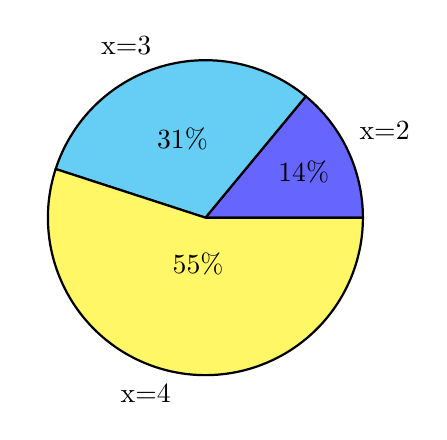
\begin{tikzpicture}

\pie[radius=2]{14/x=2,
    31/x=3,
    55/x=4}
 
\end{tikzpicture}
\caption{Pie chart for $f(x)$}
\label{fig:pie2_1_1}
\end{figure}

\begin{table}[h!]
\centering
\begin{tabular}{| c | c | c |}
 \hline
 $x$ & $f_1(x)$ & $P(x)$ \\ 
 \hline
 2 & 24 & $24/89 = 0.27$ \\  
 \hline
 3 & 29 & $29/89 = 0.33$ \\  
 \hline
 4 & 36 & $36/89 = 0.4$ \\  
 \hline
 $Total$ & 89 & 1 \\
\hline
\end{tabular}
\caption{Results for $f_1(x)$}
\label{table:table2_1_2}
\end{table}

\begin{figure}[h!]
    \centering
    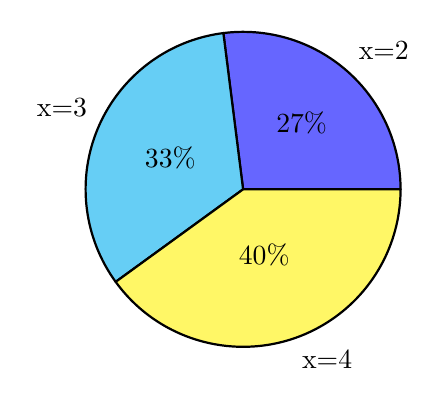
\begin{tikzpicture}
    
    \pie[radius=2]{27/x=2,
        33/x=3,
        40/x=4}
        
    \end{tikzpicture}
    \caption{Pie chart for $f_1(x)$}
    \label{fig:pie2_1_2}
\end{figure}

\subsection{}
The function $f_1$ has low selection pressure, because the probabilities for each individual are quite similar. The function $f(x)$ on the other hand applies more pressure, giving more priority to $x=4$.
\subsection{}
We can see that for scaled fitness, we have more equal probabilities for the individuals. Maybe we could use this in our favor, if we scale the fitness in the early stages of our algorithm, we would have more variability, and then we could narrow progressively the fitness to strengthen the selection pressure.

\end{document}